\subsubsection{Einflüsse auf die Routenberechnung}
\label{sec:route_explanation_definition}

\paragraph{[FR2]} NUNAV muss den \textit{End Usern} die Möglichkeit bieten, abzurufen, welche Informationen zu Verkehrsereignissen (z.B. Verkehrsfluss, Sperrungen, Baustellen, Staus) in den Algorithmus einfließen.

\bigskip

Auf der Karte, welche das Hauptinteraktionselement von \textit{NUNAV Navigation} darstellt, sind Sperrungen, Baustellen und Staus bereits eingezeichnet. Wie aus dem Nutzerfeedback hervorgeht reichen diese \textit{Context}-Informationen allerdings für das Verständnis der \textit{End User} nicht aus. Daher wurde ein neuer Hilfe-Center-Artikel im Rahmen dieser Arbeit zu diesem Thema angelegt (siehe \autoref{sec:help_center_routing_data}). Weitere Daten sind für diese statische Erklärung nicht notwendig.

Auch dieser Beitrag sollte wieder vor dem Start der Navigation erreicht werden können. Um die Standardkartenansicht nicht durch mehrere Möglichkeiten zum Aufrufen von Hilfe-Center-Artikeln zu überladen, wurde die Möglichkeit in die Routen-Vorschau integriert. Auch für diese wurden mehrere Prototypen erstellt, wobei bei der finalen Entscheidung darauf geachtet wurde, dass die Aufrufmöglichkeit nicht zu viel Platz einnimmt und der Text neugierig macht. Die verschiedenen Prototypen sind in \autoref{fig:prototype_routing_explanation} abgebildet.

\begin{figure}[htb!]
    \centering
    \subfloat[1. Prototyp zur Positionierung des Aufrufs der Erklärung]
    {
        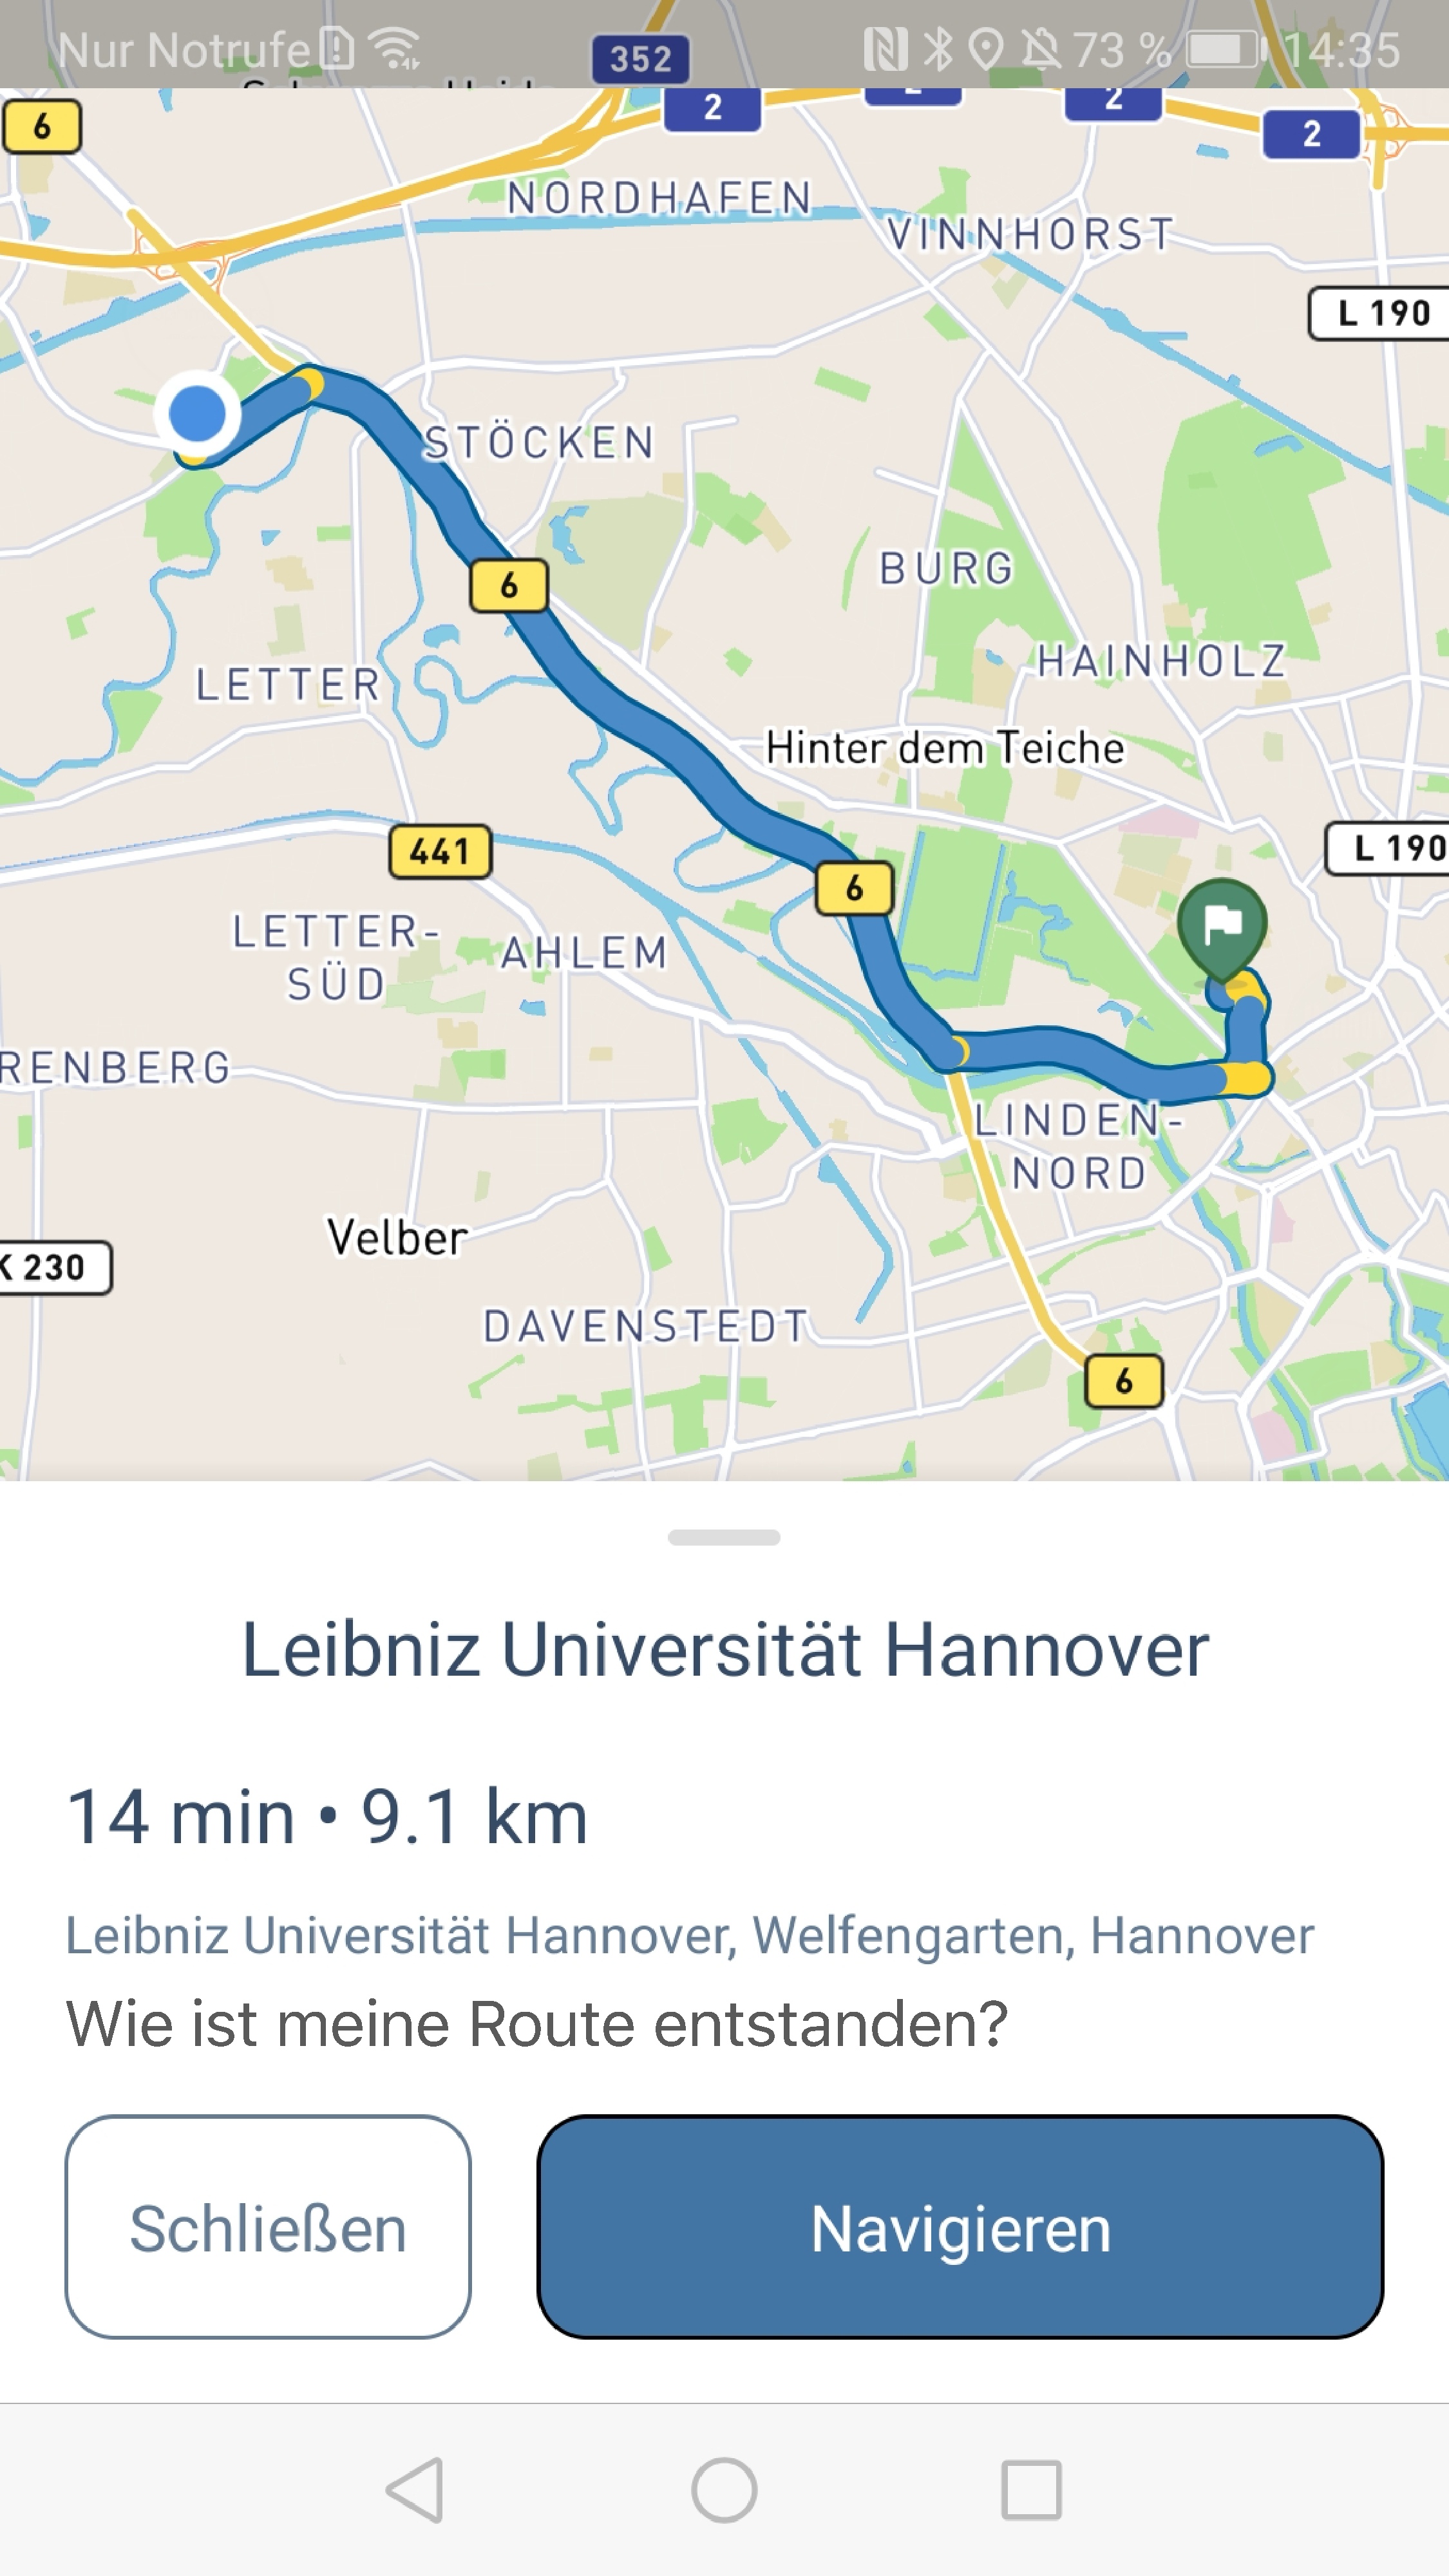
\includegraphics[width=.27\linewidth]{contents/06_model_evaluation/01_integration/res/02_routing_algorithm/prototype_1.pdf}
    }
    \hspace{.055\linewidth}
    \subfloat[Alternativer Prototyp zur Positionierung des Aufrufs der Erklärung]
    {
        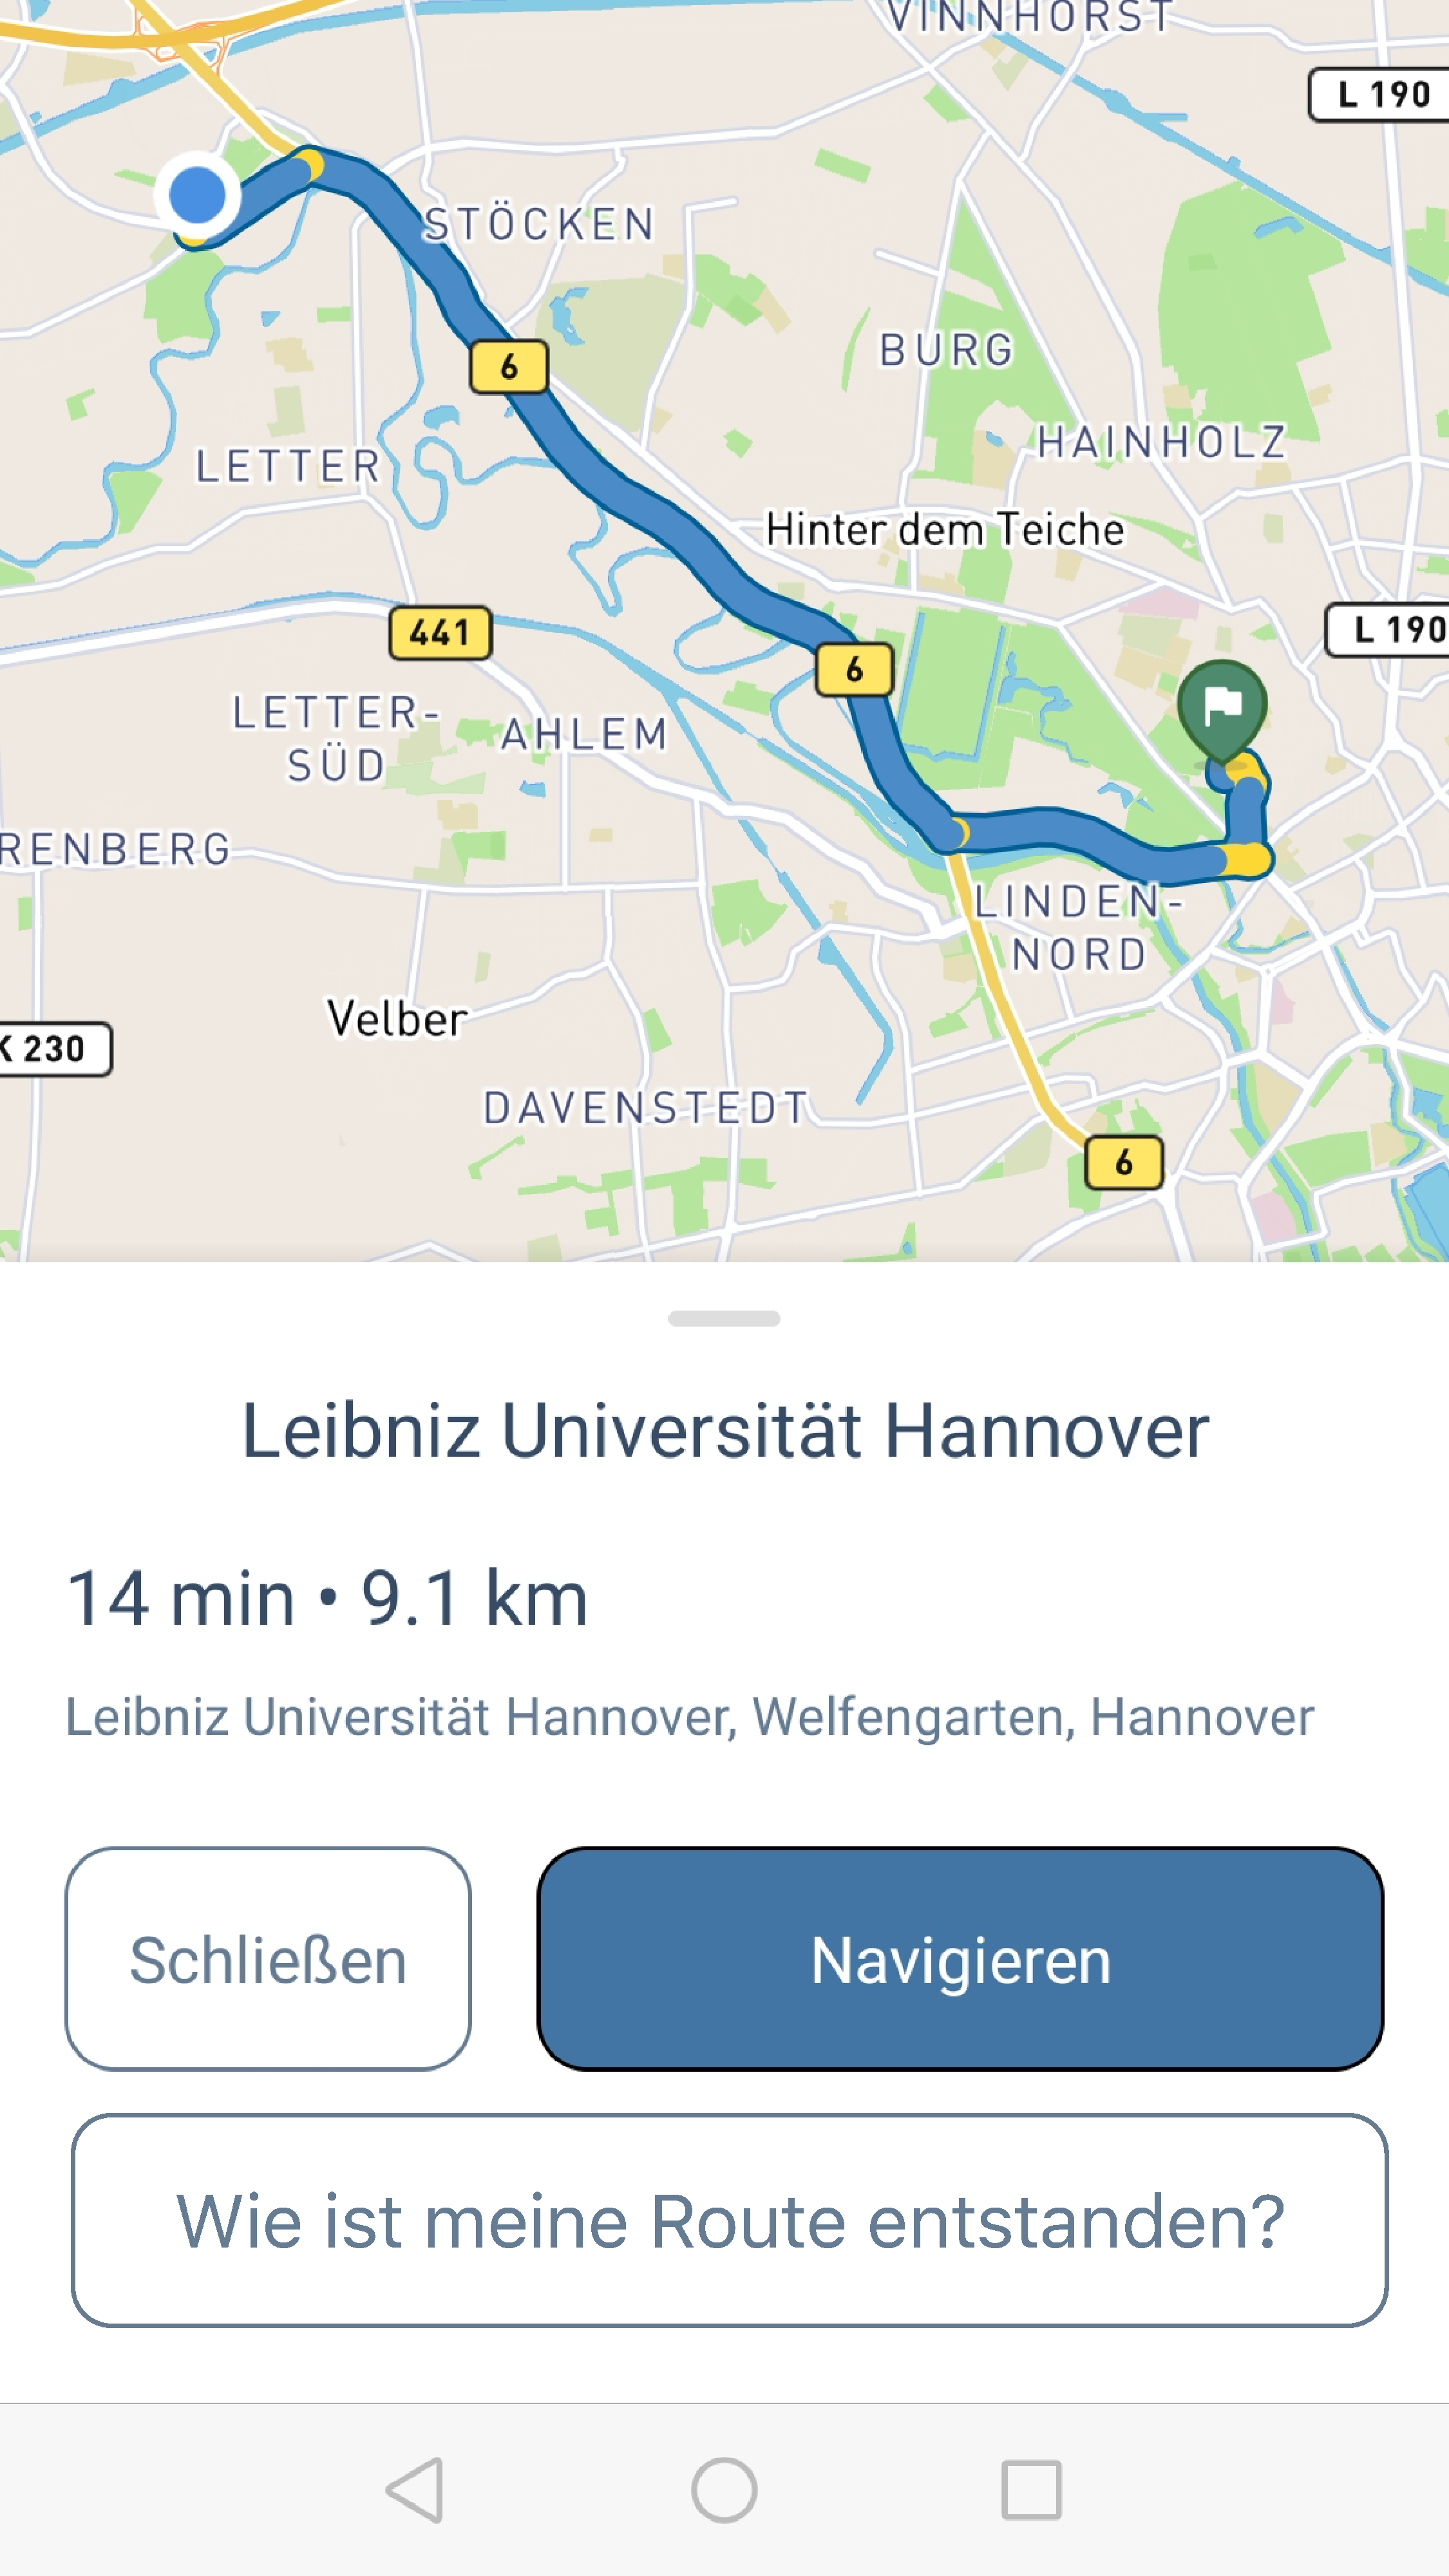
\includegraphics[width=.27\linewidth]{contents/06_model_evaluation/01_integration/res/02_routing_algorithm/prototype_2.pdf}
    }
    \hspace{.055\linewidth}
    \subfloat[Finales Design zur Positionierung des Aufrufs der Erklärung]
    {
        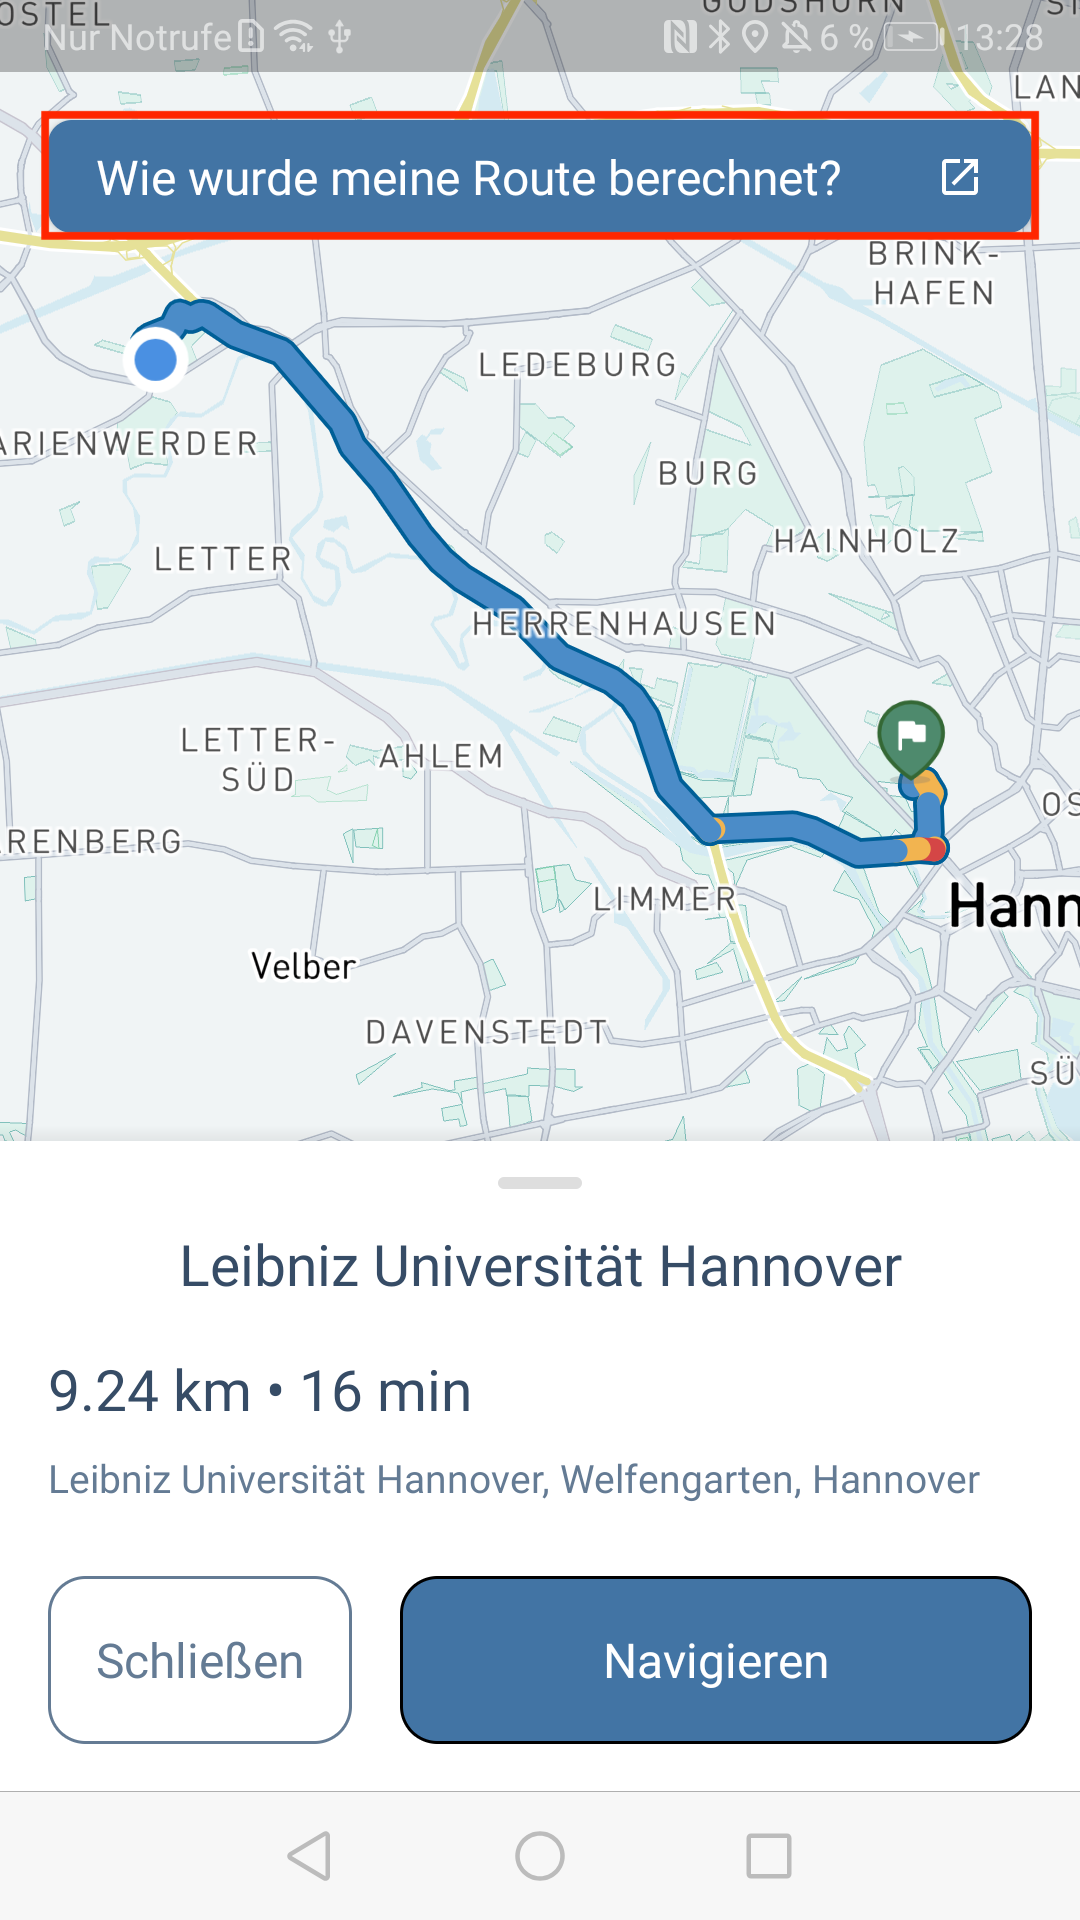
\includegraphics[width=.27\linewidth]{contents/06_model_evaluation/01_integration/res/02_routing_algorithm/final_1.png}
    }
    \caption{Prototyp und finale Designs den Aufruf der Erklärung zu Routinge-Einflüssen}
    \label{fig:prototype_routing_explanation}
\end{figure}